\documentclass[tikz,border=10pt]{standalone}
\usetikzlibrary{calc}
% Scale: 0.014981 cm per px, origin at A, y flipped
\begin{document}
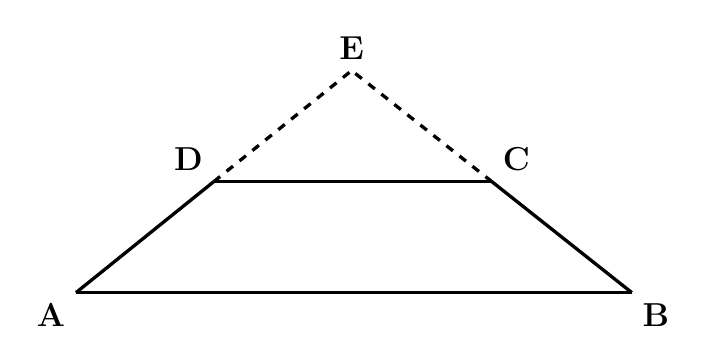
\begin{tikzpicture}[line join=round, line width=1.2pt]
  % Vertices (CV-derived, unchanged)
  \coordinate (A) at (0,0);
  \coordinate (B) at (7.059,0);
  \coordinate (C) at (5.283,1.408);
  \coordinate (D) at (1.748,1.408);
  % Apex: intersection of extended legs AD and BC
  \coordinate (E) at (3.501,2.820);

  % Solid trapezoid sides (heavier stroke, about 1.2pt)
  \draw[line width=1.2pt] (A) -- (B);
  \draw[line width=1.2pt] (D) -- (C);
  \draw[line width=1.2pt] (A) -- (D);
  \draw[line width=1.2pt] (B) -- (C);

  % Dashed extensions of the legs up to the apex (same weight)
  \draw[dashed, line width=1.2pt] (D) -- (E);
  \draw[dashed, line width=1.2pt] (C) -- (E);

  % Labels (bold math, same size)
  \node[below left] at (A) {\fontsize{12}{14.4}\selectfont $\mathbf{A}$};
  \node[below right] at (B) {\fontsize{12}{14.4}\selectfont $\mathbf{B}$};
  \node[above right] at (C) {\fontsize{12}{14.4}\selectfont $\mathbf{C}$};
  \node[above left] at (D) {\fontsize{12}{14.4}\selectfont $\mathbf{D}$};
  \node[above] at (E) {\fontsize{12}{14.4}\selectfont $\mathbf{E}$};
\end{tikzpicture}
\end{document}